\documentclass[a4paper, openright, 12pt]{article}
\usepackage[spanish]{babel}
\usepackage[utf8]{inputenc}
\usepackage{setspace}
\usepackage{url}
\usepackage{hyperref}
\usepackage{enumerate}
\usepackage{blindtext}
\usepackage{graphicx}
\usepackage{listings}
\usepackage{color}
\graphicspath{ {../imgs/} }

\author{Grupo de trabajo PAPIME}
\date{MAYO 2017}

\definecolor{codegreen}{rgb}{0,0.6,0}
\definecolor{codegray}{rgb}{0.5,0.5,0.5}
\definecolor{codepurple}{rgb}{0.58,0,0.82}
\definecolor{backcolour}{rgb}{0.95,0.95,0.92}

\lstdefinestyle{mystyle}{
    backgroundcolor=\color{backcolour},
    commentstyle=\color{codegreen},
    keywordstyle=\color{magenta},
    numberstyle=\tiny\color{codegray},
    stringstyle=\color{codepurple},
    basicstyle=\footnotesize,
    breakatwhitespace=false,
    breaklines=true,
    captionpos=b,
    keepspaces=true,
    numbers=left,
    numbersep=5pt,
    showspaces=false,
    showstringspaces=false,
    showtabs=false,
    tabsize=2
}

\lstset{style=mystyle}


\begin{document}


\begin{titlepage}

    \begin{center}
        \vspace{-1in}
        \vspace{0.35in}

        \begin{large}
            UNIVERSIDAD NACIONAL AUTÓNOMA DE MÉXICO
            \vspace{0.70in}

            FACULTAD DE PSICOLOGÍA
            \vspace{0.90in}

            CURSO DE INTRODUCCIÓN A LA PROGRAMACIÓN EN
            \textit{PYTHON}

            \vspace{4.0in}
            \rule{110mm}{0.02mm}


            \vspace{0.25in}
            JUNIO 2017

            \vspace{0.20in}
            Edgar de Jesús Vázquez Silva\\
            Laboratorio 25, Facultad de Psicología


        \end{large}


    \end{center}

\end{titlepage}


\tableofcontents
\newpage{}


%###########################
%##########################
  \section{Introducción}
    Este documento tiene la finalidad de ayudar a los alumnos de psicología a entender la estructura de un programa en Python, crear un programa básico, además de conocer algunas librerías útiles, por ejemplo: generación de gráficos.

  \newpage{}


% ###################
% ###################
  \section{Conociendo Python}
    Como estudiantes, profesores o curiosos de la programación hemos de buscar un lenguaje de programción que nos sea útil según nuestras necesidades. Es importante mencionar que existen muchos, y muy diversos, lenguajes de programación: R, Ruby, Java, Python, C, C++, por mencionar algunos. Cada uno de ellos ofrece características que lo hacen destacar según las necesidades del desarrollador.\\

    Para comenzar a programar en Python necesitaremos una interfaz que nos facilite la tarea de generar "Códigos" (programas computacionales), lo más recomendable para las personas que no han tenido un acercamiento a un lenguaje de programación es utilizar una \textit{interfaz gráfica conocida como IDLE.} Otra opción es utilizar un editor de texto como SublimeText, NotePad++ ó Atom, y ejecutarlo desde la consola. Se recomienda al lector consultar la guía de instalación del IDLE Spyder, desarrollado por los alumnos del LAB 25. \url{https://github.com/Lab25UNAM/PAPIME2016/blob/master/guia_Instalacion.pdf}\\

    En  los  siguientes  ejemplos,  las  entradas  y  salidas  son distinguidas  por  la  presencia  o  ausencia  de  los prompts \textbf{$>>>$}:  para  reproducir  los  ejemplos,  debes  escribir  todo  lo  que  esté  después  del prompt, cuando este aparezca; las líneas que no comiencen con el prompt son las salidas del intérprete.\\

    Una vez instalado la suite de desarrollo Anaconda, buscaremos el entorno de desarrollo \textit{Spyder.} Con esto estaremos listos para comenzar a desarrollar programas en lenguaje de programación Python.\\

    \subsection{Escribiendo un hola mundo}

    Una práctica muy conocida en el mundo de programación es comenzar a escribir un programa de bienvenida al lenguaje de programación. Para ello seguiremos estos sencillos pasos:

    \begin{itemize}
      \item{Buscar Anaconda en en menú inicio del sistema.}
      \item{Abrir el IDE Spyder.}
        \begin{figure}[ht]
            \centering
            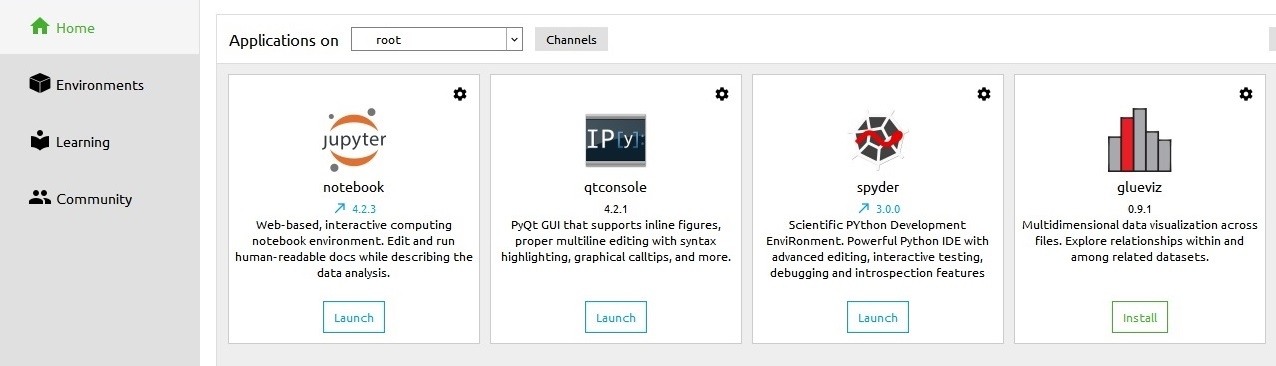
\includegraphics[width=10.5cm, height=3.5cm]{w_11.jpg}
        \end{figure}
      \item{Una vez en editor de Spyder, escribir el siguiente comando.}
    \end{itemize}


    \begin{lstlisting}[language=Python]
      print "Hola mundo...."
    \end{lstlisting}

    Con lo cual observaremos en la terminal del editor el mensaje anteriormente escrito.




  \newpage{}




  \section{Variables}
    Una de las características más poderosas en un lenguaje de programación es la capacidad de manipular variables. Se entiende como variable el nombre dado a un valor.\\

    La sentencia de asignación crea nuevas variables y les da valores:

    \begin{lstlisting}[language=Python]
mensaje = "Hola mundo.... :)"
n = 17
pi = 3.14159
    \end{lstlisting}

    Este ejemplo hace tres asignaciones. La primera asigna la cadena \textit{"Hola mundo.... :)"} a una nueva variable denominada mensaje. La segunda le asigna el entero 17 a n, y la tercera le da el valor decimal 3.14159 a pi.\\

    \subsection{Tipos de variables}
        Hasta este punto ya hemos declarado algunas variables; sin embargo es importante conocer que tipo de valores podemos asignar a estas variables. Dentro de los tipos de datos principales que podemos utilizar en Python estan:\\

        \begin{itemize}
          \item{Boleanos (bool): Son tipos de datos que solo pueden tomar dos valores True o False (Verdader o Falso). Este tipo de variables nos pueden ayudar a guardar información que responda a una pregunta de afirmación. Por ejemplo, ¿Una persona es mayor de edad?, ¿Aún hay leche en el refrigerador? ¿Una paloma ha presionado el botón azul?, etc.}
          \item{Enteros (int): Se refiere a los tipos de datos que podemos representar con un numero entero. Por Ejemplo el numero de hermanos que una persona puede tener.}
          \item{Flotantes (float): Los tipos de datos flotantes se refieren a valores numéricos con punto decimal, Por ejemplo para almacenar el valor de la estatura de una persona utilizaremos una varible de tipo flotante.}
          \item{Cadenas (string): Son tipos de datos que se refieren a un conjunto de caracteres. Este tipo de datos son muy utilizados para manejo de textos, por ejemplo despliegue de mensajes o información.}
          \item{Arreglos (Arrays): Este tipo de datos en realidad es una extensión de los anteriores, y se refiere a la forma en que organizamos los datos. Un arreglo es un acomodo especial de datos de forma contigua, a la cual accedemos mediante un indice.
          Por ejemplo, si queremos guardar las calificaciones de 25 alumnos es más conveniente hacerlo en un arreglo de flotantes llamado "calificaciones" en lugar de declarar 25 variables de tipo flotante.}
        \end{itemize}

        Muchos  de  los  ejemplos  de  este  manual,  incluso  aquellos  ingresados  en  el  prompt,  incluyen comentarios.  Los  comentarios  en  Python  comienzan  con  el  carácter  numeral, \# ,  y  se  extienden  hasta  el final  físico  de  la  línea.  Un  comentario  quizás  aparezca  al  comienzo  de  la  línea  o  seguidos  de  espacios blancos  o  código,  pero  sin  una  cadena  de  caracteres. Ya  que  los  comentarios  son  para  aclarar  código  y  no  son interpretados por Python, pueden omitirse cuando se escriben ejemplos.\\

    \begin{lstlisting}[language=Python]
# Ejemplo de tipos de datos y la declaracion de variables
# Este es un comentario, debe comenzar con el simbolo #

paloma_boton_azul = True    # Variable tipo booleana
numero_mascotas = 3         # Variable de tipo entero
promedio = 7.56             # Variable de tipo flotante
Saludo = "Hola humano... :)"# Variable de tipo cadena


#Variable de tipo arreglo
calificaciones = [8.7, 9.7, 8.9, 8.1, 7.5, 6.8]
    \end{lstlisting}

    \newpage{}




  \section{Estructuras de control condicionales}
    Una sentencia de control condicional es una estructura de programación que nos permite evaluar si una expresión es verdadera. Este tipo sentencias se emplean para responder una pregunta y tomar una desición en caso que esta sea verdadera o falsa.

    \subsection{if-else}
      La más simples de estas estructuras es la sentencia \textit{if}. Esta sentencia evalua una condicion presentada.\\

\begin{lstlisting}[language=Python]
if expresion_1 = = expresion_2:
    hacerAlgo()
\end{lstlisting}

    \vspace{0.15in}
    Para hablar de estructuras de control de flujo en Python, es imprescindible primero, hablar de identación. \textbf{¿Qué es la identación?} En un lenguaje informático, la identación es lo que la sangría al lenguaje humano escrito (a nivel formal).\\

    Así como para el lenguaje formal, cuando uno redacta una carta, debe respetar ciertas sangrías, los lenguajes informáticos, requieren una identación. No todos los lenguajes de programación, pero en el caso de Python, la identación es obligatoria, ya que de ella, dependerá su estructura.\\

    \textbf{Una identación de 4 (cuatro) espacios en blanco, indicará que las instrucciones identadas, forman parte de una misma estructura de control.}\\

\begin{lstlisting}[language=Python]
if expresion_1 = = expresion_2:
    leerVariable          # Esto pasara si la comparacion
    compararVariable      # de varibles es verdadera
    imprimirMensaje
    multiplicarVariables

imprimirMensajeFinal      # Esto ya no forma parte de la
                          # estructura   if
\end{lstlisting}

    En este ejemplo podemos observar que se verifica que la expresión\_1 sea igual que la expresión\_2. En caso de ser afirmativa la respuesta se ejecutarán las instrucciones indicadas por la \textbf{identación}. \textit{Es importante señalar que en este primer ejemplo, cuando las expresiones NO son iguales no se toma ninguna acción.} Esta observación es importante; pues esta primera estructura nos servirá cuando queremos evaluar una condicion y solo nos importen tomar acción en ese caso.\\

    A continuación se enuncia un ejemplo en el cual nos interesa realizar una acción cuando las sentencias sean verdaderas y otro acción diferente cuando la sentencia NO sea verdadera.\\


    La estrcutura if-else por su parte ofrece una alternativa de acción en caso que la sentecia a comparar sea falsa. Esta estructura puede declararse como se muestra a continuación:\\

\begin{lstlisting}[language=Python]
if expresion_1 = = expresion_2:
    leerVariable          # Esto pasara si la comparacion
    compararVariable      # de varibles es verdadera
    imprimirMensaje
    multiplicarVariables
else
    imprimirMensaje       # Esto pasara si la comparacion
    terminarPrograma      # es falsa

imprimirMensajeFinal      # Esto ya no forma parte de la
                          # estructura   if
\end{lstlisting}


    Como observamos en el ejemplo 2, primero evaluaremos que la expresión\_1 y la expresion\_2 sean iguales, si ocurre el caso en que ambos tengan el mismo valor se ejecutará la secuencia de pasos número\_1; en el caso contrario cuado la expresión\_1 y la expresión\_2 \textbf{NO} sean iguales se ejecutará la secuencia de pasos número\_2.\\

    Con la finalidad de ser más claro con el lector a continuación se mencionan algunos ejemplos.\\

\begin{lstlisting}[language=Python]
# En este primer caso solo nos interesa realizar
# una accion cuando la sentencia sea verdadera
# Por lo tanto no lleva condicional else

if velocidadAutomovil > 90:
    multarCondutor
\end{lstlisting}

    En este primer caso no es relevante saber si el conductor va a una velocidad menor que la límite.\\

\begin{lstlisting}[language=Python]
# En este segundo caso nos interesa realizar
# una accion cuando la sentencia sea verdadera
# y otra accion cuando sea diferente

if velocidadAutomovil > 90:
    if edadConductor > 18:
        multarConductor
    else
        llamarAlosPadres
\end{lstlisting}

  En este ejemplo, nos interesa saber dos cosas: si el automóvil va a una velocidad mayor que la límite (en este caso 90 km/h) y si el conductor es menor o mayor de edad.\\

  Hasta ahora ya hemos visto como preguntar si dos expresiones son iguales; sin embargo hay más comparaciones que podemos realizar. A continuación se enlistan los comparadores más comunes en Python.\\



\begin{center}
  \begin{tabular}{ |c|c|c|c| }
    \hline
      \textbf{Simbolo}&\textbf{Significado} & \textbf{Ejemplo} & \textbf{Resultado} \\
      ==    & igual que      &    89 == 7       & Falso\\
      !=    & diferente      &    verde != rojo & Verdadero\\
      $<$   & menor que      &    12.0 $<$ 12.5   & Verdadero\\
      $>$   & mayor que      &    8 $>$ 10        & Falso\\
      $<=$  & menor o igual que & 12 $<=$ 12      & Verdadero\\
      $>=$  & mayor o igual que & 15 $>=$ 20      & Falso\\
    \hline
  \end{tabular}
\end{center}

    \newpage{}


  \section{Ciclos condicionales}
    A diferencia de las estructuras de control condicionales, las iterativas (también llamadas cíclicas o bucles), nos permiten \textit{ejecutar un mismo código, de manera repetida}, mientras se cumpla una condición.\\

    En Python se dispone de dos estructuras cíclicas:

    \begin{itemize}
      \item{El bucle while}
      \item{El bucle for}
    \end{itemize}

    Las veremos en detalle a continuación.\\

    \subsection{Ciclo while}
      Este bucle, se encarga de ejecutar una misma acción \textbf{“mientras que”} una determinada condición se cumpla.\\

      Ejemplo: \textit{Mientras que año sea menor o igual a 2017, imprimir la frase "Informe del año \_anio\_"}\\

\begin{lstlisting}[language=Python]
#Declaramos e inicializamos una variable
anio = 2000

while anio <= 2017:
  print "Informe del ciclo ", str(anio)
  anio = anio+1
\end{lstlisting}

    Podemos notar que el ciclo while repetirá la impresión de un mensaje mientras que el valor de la variable anio sea menor o igual que 2017; además de realizar esta acción realizamos una acción más, el incremento de la variable en una unidad. \textbf{¿Que pasrá si no se incrementa esta variable?} la variable anio siempre tendrá un valor de 2000 y nunca saldrá del ciclo \textit{while}. El ejemplo anterior tendrá una salida similar a esta:\\

\begin{lstlisting}[language=Python]
Informe del ciclo 2000
Informe del ciclo 2001
Informe del ciclo 2002
Informe del ciclo 2003
Informe del ciclo 2004
.
.

.
Informe del ciclo 2017
\end{lstlisting}

    Pero, ¿Que sucede si el ciclo while es infinito o demasiado largo? Por ejemplo deseamos realizar un programa que pregunte al usuario su nombre y si la persona se llama $"$Eduardo$"$ imprimiremos un mensaje de felicitación. Para resolver situaciones de este tipo se emplea la instrucción $"break"$.\\

\begin{lstlisting}[language=Python]
while True:
  nombre = raw_input("Indica tu nombre:  ")
  if nombre == "Eduardo" :
    break

print "Hola Eduardo, bienvenido al sistema..."
\end{lstlisting}

    En este caso el ciclo while se repetirá infinitamente. El ciclo consiste en preguntar el nombre de una persona y lo guarda en una variable llamada $"nombre"$, posteriormente verifica si el valor de la variable es igual a $"Eduardo"$, si la respuesta es afirmativa va a instrucción \textit{break} y sale del ciclo while. En caso que el nombre no sea igual a $"Eduardo"$ el programa seguirá ejecutando el ciclo while, preguntando infinitamente.\\


    \subsection{ciclo for}
      El ciclo for en el lenguaje Python tiene cierta ventaja y diferencia con otros lenguajes. Podemos pensar que el ciclo For se define utilizando contadores y rangos en los cuales se ejecutaría el código del for.\\

      A continuación la sintaxis de For en Python.\\

La sintaxis es la siguiente:\\
\begin{lstlisting}[language=Python]
  for iterador in secuencia
       #codigo a ejecutar
\end{lstlisting}


    Esto quiere decir que cuando usamos la sentencia For, tenemos la capacidad de recorrer una secuencia por medio de “iteraciones”, una secuencia como una lista o una simple cadena de texto, veamos un ejemplo para comprender mejor.\\

    Si quisiéramos declarar una cadena de texto y recorrer cada uno de sus caracteres, podemos usar la sentencia For para ello.\\

    Este programa recorrera cada letra de la cadena de texto “Hola!” y la imprimira en pantalla.\\

    \begin{lstlisting}[language=Python]
#!/usr/bin/python

for letra in 'Hola!':
  print 'Estamos en la letra :', letra


Este seria el resultado:
Estamos en la letra : H
Estamos en la letra : o
Estamos en la letra : l
Estamos en la letra : a
Estamos en la letra : !
    \end{lstlisting}


    \subsubsection{Iterar utilizando Indices (listas)}

    También es posible hacer iteraciones con For utilizando indices de listas. Esto quiere decir que la variable iterada tendra el valor de un indice, algo así como un contador común y corriente.\\

    Ejemplo:\\

    \begin{lstlisting}[language=Python]
#!/usr/bin/python
autos = ['mercedez','BMW','Toyota']

for indice in range(len(autos)) #range define un rango que es el tamano de la lista
       print 'El auto es un ',autos[indice]



En este ejemplo iteramos una lista de autos y  los accedemos utilizando el indice de la lista, el resultado seria:

El auto es un mercedez
El auto es un BMW
El auto es un Toyota



La equivalencia sin usar el indice seria la siguiente:
#!/usr/bin/python

autos = ['mercedez','BMW','Toyota']

for auto in autos
  print 'El auto es un ',auto
    \end{lstlisting}


    En cuyo caso la variable “auto” esta iterando la secuencia de la lista de autos, y toma el valor de cada uno de sus elementos dentro de esta lista.\\

    \newpage{}

  \section{Definición de funciones}
    En Python, la definición de funciones se realiza mediante la instrucción \textbf{def} más un nombre de función descriptivo para el cuál, aplican las mismas reglas que para el nombre de las variables seguido de paréntesis de apertura y cierre. Como toda estructura de control en Python, la definición de la función finaliza con dos puntos (:) y el algoritmo que la compone, irá identado con 4 espacios:\\

\begin{lstlisting}[language=Python]
def mi_funcion():
    # aqui el algoritmo
\end{lstlisting}

\textbf{Una función, no es ejecutada hasta tanto no sea invocada. Para invocar una función, simplemente se la llama por su nombre:}\\

\begin{lstlisting}[language=Python]
def mi_funcion():
    print "Hola Mundo"

funcion()
\end{lstlisting}

Cuando una función, haga un retorno de datos, éstos, pueden ser asignados a una variable:\\

\begin{lstlisting}[language=Python]
def funcion():
    return "Hola Mundo"

frase = funcion()
print frase
\end{lstlisting}



    \subsubsection{Sobre los parámetros}

    Un parámetro es un valor que la función espera recibir cuando sea llamada (invocada), a fin de ejecutar acciones en base al mismo. Una función puede esperar uno o más parámetros (que irán separados por una coma) o ninguno.\\

\begin{lstlisting}[language=Python]
def mi_funcion(nombre, apellido):
    # algoritmo
\end{lstlisting}

    Los parámetros, se indican entre los paréntesis, a modo de variables, a fin de poder utilizarlos como tales, dentro de la misma función.\\

    Los parámetros que una función espera, serán utilizados por ésta, dentro de su algoritmo, a modo de variables de ámbito local. Es decir, que los parámetros serán variables locales, a las cuáles solo la función podrá acceder:


\begin{lstlisting}[language=Python]
def mi_funcion(nombre, apellido):
    nombre_completo = nombre, apellido
    print nombre_completo
\end{lstlisting}


    En Python, también es posible, asignar valores por defecto a los parámetros de las funciones. Esto significa, que la función podrá ser llamada con menos argumentos de los que espera:\\

\begin{lstlisting}[language=Python]
def saludar(nombre, mensaje='Hola'):
    print mensaje, nombre

saludar('Pepe Grillo') # Imprime: Hola Pepe Grillo
\end{lstlisting}

    \newpage{}


  \section{Librerías}
    \subsection{numpy}
    \subsection{matplotlib}
    \subsection{scipy}


\end{document}